\section{Generators}

By sequentially or horizontally composing the \textit{Z Spider} (green) and \textit{X Spider} (red) generators, we can construct undirected multigraphs known as ZX diagrams \cite{Wetering2020}. That is, graphs that allow multiple edges between vertices. Since \textit{only connectivity matters} in the ZX calculus, a valid ZX diagram can be deformed as seen fit, provided that the order of inputs and outputs is preserved.
\begin{figure}[H]
\centering
    \centering
    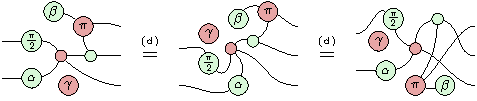
\includegraphics[width=0.8\textwidth]{chapter-2/connectivity}
    \caption{Three equivalent ZX diagrams (\textit{only connectivity matters}).}
\end{figure}

Z Spiders are defined with respect to the $Z$ eigenbasis such that a Z Spider with $n$ inputs and $m$ outputs has the following interpretation as a linear map. Note that in this text, we will interpret the flow of time from left to right.
\begin{figure}[H]
\centering
\includezxdiagramtext{figures/chapter-2/z_spider}{0.21}{\,
    \ket{0}^{\otimes m} \bra{0}^{\otimes n} + e^{i\alpha}
    \ket{1}^{\otimes m} \bra{1}^{\otimes n}}
\caption{Interpretation of Z Spider as a linear map.}
\end{figure}
Similarly, X Spiders, which are defined with respect to the $X$ eigenbasis, are interpreted as the following linear map.
\begin{figure}[H]
\centering
\includezxdiagramtext{figures/chapter-2/x_spider}{0.21}{\,
    \ket{+}^{\otimes m} \bra{+}^{\otimes n} + e^{i\alpha}
    \ket{-}^{\otimes m} \bra{-}^{\otimes n}}
\caption{Interpretation of X Spider as a linear map.}
\end{figure}

We can recover the $\ket 0$ eigenstate using an X Spider that has a phase of zero, or the $\ket 1$ eigenstate using an X Spider that has a phase of $\pi$.
\begin{figure}[H]
\centering
\begin{minipage}{.4\textwidth}
    \centering
    \includezxdiagramtext{figures/chapter-2/zero_state}{0.15}{\,
        \ket + + \ket - = \sqrt{2} \ket 0}
    \caption{$\ket 0$ eigenstate}
\end{minipage}%
\begin{minipage}{.4\textwidth}
    \centering
    \includezxdiagramtext{figures/chapter-2/one_state}{0.16}{\,
    \ket + - \ket - = \sqrt{2} \ket 1}
    \caption{$\ket 1$ eigenstate}
\end{minipage}
\end{figure}

Likewise, we have the $\ket +$ and $\ket -$ basis states from the corresponding Z Spider
\begin{figure}[H]
\centering
\begin{minipage}{.4\textwidth}
    \centering
    \includezxdiagramtext{figures/chapter-2/plus_state}{0.15}{\,
        \ket 0 + \ket 1 = \sqrt{2} \ket +}
    \caption{$\ket +$ eigenstate}
\end{minipage}%
\begin{minipage}{.4\textwidth}
    \centering
    \includezxdiagramtext{figures/chapter-2/minus_state}{0.16}{\,
    \ket 0 - \ket 1 = \sqrt{2} \ket -}
    \caption{$\ket -$ eigenstate}
\end{minipage}
\end{figure}

Whilst we obtain the correct states, we obtain the wrong scalar factor. For the remainder of this thesis, we will ignore global non-zero scalar factors. Hence, equal signs should be interpreted as `equal up to a global phase'.

Single qubit rotations in the $Z$ basis are represented by a Z Spider with a single input and a single output. Arbitrary rotations in the $X$ basis are represented by the corresponding $X$ spider. We can view these as rotations of the Bloch sphere.

\begin{figure}[H]
\centering
    \includezxdiagramtextplus{figures/chapter-2/z_rotation}{0.11}{
        \ket{0} \bra{0} + e^{i\alpha} \ket{1} \bra{1} = 
    \begin{pmatrix} 1 & 0 \\ 0 & e^{i\alpha} \end{pmatrix} \rightarrow
    }{chapter-1/z_rotation}{0.18}
    %
    \includezxdiagramtextplus{figures/chapter-2/x_rotation}{0.11}{
        \ket{+} \bra{+} + e^{i\alpha} \ket{-} \bra{-} = 
        \frac{1}{2}
        \begin{pmatrix}
            1 + e^{i\alpha} & 1 - e^{i\alpha} \\
            1 - e^{i\alpha} & 1 + e^{i\alpha}
        \end{pmatrix} \rightarrow
    }{chapter-1/x_rotation}{0.17}
\caption{Arbitrary single qubit rotations in the $Z$ and $X$ bases.}
\end{figure}

We can recover the Pauli $Z$ and Pauli $X$ matrices by setting the angle $\alpha = \pi$.
\begin{figure}[H]
\centering
\includezxdiagramtext{figures/chapter-2/pauli_z}{0.11}{
    \ket{0} \bra{0} + e^{i\pi} \ket{1} \bra{1} = 
    \begin{pmatrix} 1 & \,\,0 \\ 0 & -1 \end{pmatrix}
}
\includezxdiagramtext{figures/chapter-2/pauli_x}{0.11}{
    \ket{+} \bra{+} + e^{i\pi} \ket{-} \bra{-} = 
    \begin{pmatrix} 0 & 1 \\ 1 & 0 \end{pmatrix}
}
\caption{Pauli $Z$ and $X$ gates in the ZX calculus.}
\end{figure}

%%%

\subsection{Composition}
To calculate the matrix of a ZX diagram consisting of sequentially composed spiders, we take the matrix product. Note that the order of operation of matrix multiplication is the reverse as in the ZX diagram as we have defined it.

\includezxdiagramtext{chapter-2/sequential}{0.27}{
\begin{pmatrix} 1 & 0 \\ 0 & e^{i\gamma} \end{pmatrix}
\begin{pmatrix}
    1 + e^{i\beta} & 1 - e^{i\beta} \\
    1 - e^{i\beta} & 1 + e^{i\beta}
\end{pmatrix}
\begin{pmatrix} 1 & 0 \\ 0 & e^{i\alpha} \end{pmatrix}}

Alternatively, we could have chosen to compose the spiders in parallel, resulting in the tensor product.

\includezxdiagramtext{chapter-2/parallel}{0.105}{
\begin{pmatrix} 1 & 0 \\ 0 & e^{i\alpha} \end{pmatrix} \otimes
\begin{pmatrix}
    1 + e^{i\beta} & 1 - e^{i\beta} \\
    1 - e^{i\beta} & 1 + e^{i\beta}
\end{pmatrix}}

The CNOT gate in the ZX calculus is represented by a Z spider (control qubit) and an X spider (target qubit). We can arbitrarily deform the diagram and decompose it into matrix and tensor products as follows.

\includezxdiagram{chapter-2/cnot_def}{0.65}

We can calculate matrix $A$, consisting of a single-input and two-output Z Spider ($4 \times 2$ matrix) and an empty wire (identity matrix), by taking the tensor product.

\includezxdiagramtext{chapter-2/A_def}{0.33}{
\begin{pmatrix}
    1 & 0 \\
    0 & 0 \\
    0 & 0 \\
    0 & 1
\end{pmatrix} \otimes
\begin{pmatrix} 1 & 0 \\ 0 & 1 \end{pmatrix}}

Similarly, to calculate the matrix $B$, we take the following tensor product.

\includezxdiagramtext{chapter-2/B_def}{0.33}{
\begin{pmatrix} 1 & 0 \\ 0 & 1 \end{pmatrix} \otimes \frac{1}{\sqrt 2}
\begin{pmatrix} 1 & 0 & 0 & 1 \\ 0 & 1 & 1 & 0 \end{pmatrix}}

We can then calculate the CNOT matrix by taking the matrix product of matrix $A$ and matrix $B$ as follows.

\includezxdiagramtext{chapter-2/cnot}{0.10}{
\Bigg[
\begin{pmatrix} 1 & 0 \\ 0 & 1 \end{pmatrix} \otimes \frac{1}{\sqrt 2}
\begin{pmatrix} 1 & 0 & 0 & 1 \\ 0 & 1 & 1 & 0 \end{pmatrix} \Bigg]
%
\left[ \begin{pmatrix}
    1 & 0 \\
    0 & 0 \\
    0 & 0 \\
    0 & 1 \\
\end{pmatrix} \otimes
\begin{pmatrix} 1 & 0 \\ 0 & 1 \end{pmatrix} \right] \simeq
%
\begin{pmatrix}
1 & 0 & 0 & 0 \\
0 & 1 & 0 & 0 \\
0 & 0 & 0 & 1 \\
0 & 0 & 1 & 0
\end{pmatrix}}

Had we chosen to make the first qubit the target and the second qubit the control, we would have obtained the following.
\includezxdiagramtext{chapter-2/cnot2}{0.10}{
\Bigg[
\frac{1}{\sqrt 2}
\begin{pmatrix} 1 & 0 & 0 & 1 \\ 0 & 1 & 1 & 0 \end{pmatrix} \otimes 
\begin{pmatrix} 1 & 0 \\ 0 & 1 \end{pmatrix}
\Bigg]
%
\left[
\begin{pmatrix} 1 & 0 \\ 0 & 1 \end{pmatrix} \otimes
\begin{pmatrix} 1 & 0 \\ 0 & 0 \\ 0 & 0 \\ 0 & 1 \end{pmatrix}
\right] \simeq
%
\begin{pmatrix}
1 & 0 & 0 & 0 \\
0 & 1 & 0 & 0 \\
0 & 0 & 0 & 1 \\
0 & 0 & 1 & 0
\end{pmatrix}}

Since \textit{only connectivity matters}, we could have equivalently calculated the matrix of the CNOT gate by deforming the diagram as follows.

\vspace{10pt}
\includezxdiagram{chapter-2/cnot_def2}{0.65}

\subsection{Hadamard Generator}

All quantum gates are unitary transformations. Therefore, up to a global phase, an arbitrary single qubit rotation $U$ can be viewed as a rotation of the Bloch sphere about some axis. We can decompose the unitary $U$ using Euler angles to represent the rotation as three successive rotations \cite{Wetering2020}.
\begin{figure}[H]
    \centering
    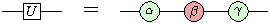
\includegraphics[width=0.5\textwidth]{chapter-2/unitary}
    \caption{Arbitrary single-qubit rotation.}
\end{figure}

Recall that the Hadamard gate $H$ switches between the $\ket 0$/$\ket 1$ and $\ket +$/$\ket -$ bases. That is, it corresponds to a rotation of the Bloch sphere by $\pi$ radians about the line bisecting the $X$ and $Z$ axes. By choosing $\alpha = \beta = \gamma = \frac{\pi}{2}$, we obtain the Hadamard gate up to a global phase of $e^{-i\frac{\pi}{4}}$. We define the Hadamard generator below.

\begin{figure}[H]
    \includezxdiagramtextplus{figures/chapter-2/hadamard}{0.56}{
    % \frac{1}{\sqrt 2} \begin{pmatrix} 1 & 1 \\ 1 & -1 \end{pmatrix} \rightarrow
    }{chapter-1/hadamard}{0.16}
    \caption{Hadamard generator in the ZX calculus.}
\end{figure}

There are many equivalent ways of decomposing the Hadamard gate using Euler angles. Note that the rightmost representations need no scalar corrections.
\begin{figure}[H]
\centering
    \centering
    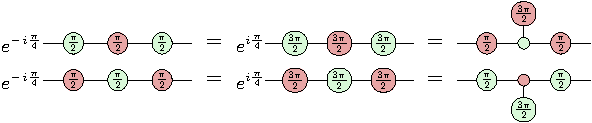
\includegraphics[width=1\textwidth]{chapter-2/hadamard_decomp}
    \caption{Equivalent definitions of the Hadamard generator.}
\end{figure}

\subsection{Conjugate, Transpose and Adjoint}

We can find the conjugate of a ZX diagram by simply negating the phases of all spiders in the diagram, $\alpha \rightarrow -\alpha, \,\, \beta \rightarrow -\beta, \dots$.

\includezxdiagram{chapter-2/conjugate}{0.6}

We can find the transpose of a ZX diagram by turning all of its inputs into outputs and all of its outputs into inputs.

\includezxdiagram{chapter-2/transpose}{1}

It is then a simple matter to find the Hermitian adjoint of a ZX diagram by first finding its conjugate, then its transpose.

\includezxdiagram{chapter-2/adjoint}{0.6}

